\documentclass[10pt,twocolumn]{article}  % JNeurosci published-article look
\usepackage{jneurosci}
\bibliographystyle{jneurosci-etal}  % jneurosci.bst for full author lists
\usepackage{url}
\usepackage{amsmath}
\usepackage{iftex}
\ifPDFTeX
  \usepackage{pxfonts}
  \usepackage[T1]{fontenc}
  \usepackage[utf8]{inputenc}
\else  % XeTeX (tectonic): Palatino clone with Unicode support
  \usepackage{fontspec}
  \setmainfont{texgyrepagella}[Extension=.otf, UprightFont=*-regular, BoldFont=*-bold,
    ItalicFont=*-italic, BoldItalicFont=*-bolditalic]
  \setsansfont{texgyreheros}[Extension=.otf, UprightFont=*-regular, BoldFont=*-bold,
    ItalicFont=*-italic, BoldItalicFont=*-bolditalic, Scale=MatchLowercase]
  \usepackage{unicode-math}
  \setmathfont{texgyrepagella-math.otf}
\fi
\usepackage{xcolor}
\usepackage{setspace}
\usepackage{lineno}
\usepackage{graphicx}
\graphicspath{{img/}{paper/img/}}  % figures found whether compiled from paper/ or the repo root (Overleaf)
\usepackage{float}
\usepackage{multicol}
\usepackage{tikz}
\usetikzlibrary{decorations.pathreplacing}
\usepackage{ragged2e}
\usepackage{etoolbox}
\AtBeginEnvironment{itemize}{\RaggedRight}  % bullet lists left-aligned
\setlength{\emergencystretch}{1.5em}
\usepackage[left=0.75in,top=0.8in,right=0.75in,bottom=0.8in,columnsep=0.25in]{geometry}
\makeatletter  
\renewcommand\section{\@startsection{section}{1}{\z@}{-10pt plus -2pt minus -1pt}{4pt}{\raggedright\sffamily\bfseries\large}}
\renewcommand\subsection{\@startsection{subsection}{2}{\z@}{-8pt plus -2pt minus -1pt}{2pt}{\raggedright\sffamily\bfseries\normalsize}}
\renewcommand\subsubsection{\@startsection{subsubsection}{3}{\z@}{-6pt plus -1pt minus -1pt}{2pt}{\raggedright\sffamily\itshape\normalsize}}
\makeatother
\usepackage[font=footnotesize,labelfont=bf,labelsep=period,justification=justified,singlelinecheck=false]{caption}
\usepackage[colorlinks=true, linkcolor=black, citecolor=black, urlcolor=blue]{hyperref}
\let\citetext\relax
\usepackage{natbib}
\let\cite\citep
\renewcommand{\bibfont}{\footnotesize}  % small reference list, as in the journal
\setlength{\bibsep}{1pt}
\renewcommand{\dbltopfraction}{0.9}  % allow tall full-width figures at the top of a page
\renewcommand{\dblfloatpagefraction}{0.8}
\raggedbottom  % no vertical stretching to fill columns
\renewcommand{\bibsection}{\section*{References}}
\makeatletter  % JNeurosci title block: left-aligned, spans both columns
\renewcommand{\maketitle}{\twocolumn[{\begin{flushleft}{\LARGE\bfseries\@title\par}\vspace{8pt}%
  {\large\bfseries\@author\par}\vspace{3pt}%
  {\small Department of Psychology, University of Pennsylvania, Philadelphia, Pennsylvania\par}\end{flushleft}\vspace{10pt}%
  \ifdefined\abstracttext{\small\bfseries\noindent\abstracttext\par}\vspace{16pt}\fi}]}
\makeatother

\newcommand{\cut}{\textcolor{red}{\textbf{\,[C]}}}  
\newcommand{\new}[1]{\textcolor{blue}{#1}}  
\newcommand{\panel}[3]{% \panel{label}{width}{file}
  \begin{minipage}[t]{#2\linewidth}\vspace{0pt}\textbf{#1}\par\vspace{4pt}\includegraphics[width=\linewidth]{#3}\end{minipage}}
\newcommand{\panelc}[3]{
  \begin{minipage}[c]{#2\linewidth}\textbf{#1}\par\vspace{4pt}\includegraphics[width=\linewidth]{#3}\end{minipage}}
\providecommand{\tightlist}{\setlength{\itemsep}{0pt}\setlength{\parskip}{0pt}}


\title{Word-onset response across the human brain: timing, networks and reliability}
\author{Juee Naik, Michael Kahana}
\date{}

\begin{document}
\newcommand{\abstracttext}{Scalp EEG, MEG and fMRI studies establish the stages of visual word processing, and intracranial studies typically analyze how word-evoked activity varies with cognitive state, yet studies of the word response itself, often small and ventral-stream focused, leave network dynamics and replicability largely untested. Recording across the brain in 362 neurosurgical patients performing delayed free recall, we compare each word with the inter-stimulus interval (ISI) before it. As expected, occipital regions respond most strongly, with decreased alpha (8-13 Hz) and increased high-gamma (70-150 Hz) power, although magnitude varies widely across patients. Beyond the ventral stream, frontal regions show an alpha increase, suggesting suppression. High-gamma latencies increase from lateral occipital cortex (~120 ms) to orbitofrontal cortex (~320 ms); occipital regions reliably lead most lobes and frontal regions lag most, but adjacent lobes largely overlap. Alpha synchrony rises, with hubs shifting forward from occipital to parietal to temporal regions, while the hippocampus does not join. Despite variability across subjects, power changes within subjects are stable across sessions (median r = 0.67 alpha, 0.81 high gamma), but synchrony changes are not (0.19, 0.14); across subjects, only occipital connectivity replicates (r = 0.90). The response also carries cognitive effects: occipital responses are larger after longer ISIs, consistent with temporal expectation, and single-lobe classifiers weakly predict later recall, in frontal regions even before the response begins. These results establish where, when and how reliably the brain responds to words, a reference for interpreting cognitive effects measured during word presentation.}
\maketitle


\section*{Introduction}\label{introduction}

\subsection*{The word-onset response in free recall}\label{intro-word-onset}

Most intracranial EEG (iEEG) studies of free recall contrast words that are later recalled with words 
that are forgotten (the subsequent memory effect, SME), or study the retrieval period. 
As both conditions contain a word, this contrast measures how responses differ with later memory, 
but cancels out the response to the word itself. Only a few studies have examined the word-onset response directly. \citet{Kucewicz_2019} showed that high-gamma (HG) activity after word onset moves from visual cortex to the medial temporal lobe (MTL) and then to prefrontal cortex, and \citet{Marks_2021} found that theta, alpha/beta and gamma activity each spread across regions on their own timelines during word encoding.

\subsection*{High gamma and alpha as markers of cortical engagement }\label{intro-hg-alpha}
%(cut/reduce?)
Broadband HG (70--150 Hz) is widely used as a measure of local population spiking \citep{Manning_2009,Ray_2011}. 
At stimulus onset, alpha and beta power decrease \citep[event-related desynchronization;][]{Pfurtscheller_1999}; 
together, an alpha decrease and an HG increase mark a region engaged by a stimulus. 
Conversely, alpha increases in task-irrelevant regions are thought to mean suppression \citep{Jensen_2010}, 
so the same two measures can separate regions that a stimulus engages from regions it suppresses.

\subsection*{Timing of visual word processing}\label{intro-timing}
%(most imp.)
Reading a word progresses in stages: visual features are extracted within about 100 ms \citep{Thorpe_1996}, 
the letter string is recognised as a word at about 200 ms \citep{Cohen_2000}, its sound is activated 
automatically \citep{van_Orden_1987}, and its meaning is integrated with context by about 400 ms 
\citep{Kutas_1980}. These stages imply a reading network that runs from occipital cortex through left 
fusiform gyrus, which contains the visual word form area \citep[VWFA;][]{Cohen_2000,Dehaene_2011}, to 
temporal, supramarginal and inferior frontal cortex \citep{Price_2012,Taylor_2013}, with posterior 
responses to letter strings preceding more anterior responses to lexical status \citep{Nobre_1994,Allison_1994}. 
Much of this picture comes from scalp EEG, MEG, and fMRI, which resolve the order in which these stages 
occur but not precisely when and where, while iEEG records local activity with both 
millisecond and millimetre precision \citep{Parvizi_2018}. However, most intracranial studies of reading 
record from tens of subjects with sparse, clinically determined coverage and focus on the ventral stream, 
and so the order in which regions across the whole brain respond to a word has not been measured within one 
large dataset.

\subsection*{Synchrony, expectation and memory}\label{intro-sync-expect-memory}

Beyond local activity, word onset may change how regions synchronize. Alpha phase synchrony is thought 
to coordinate distant regions \citep{Palva_2007}, and in free recall, low-frequency synchrony between regions 
increases during successful encoding and retrieval \citep{Solomon_2017,Rao_2025}. The response may also 
depend on when the word is expected: the inter-stimulus interval (ISI) before each word varies in length, and the longer it lasts, 
the more expected the word becomes \citep{Nobre_2017}. Finally, spectral features recorded while a word 
is studied predict whether it will be recalled \citep{Ezzyat_2017}, and comparing recalled with forgotten 
words region by region, HFA predicting later recall appears first in visual, fusiform and medial 
temporal regions and later in left inferior frontal, posterior parietal and ventrolateral temporal 
cortex \citep{Burke_2014a}. These approaches either pool features across the brain and the whole word 
period, or test each region and time point for a difference in mean activity. How well each region's 
single-event response predicts recall, and when that prediction arises, has not been measured with 
classifiers.

\subsection*{The present study }\label{intro-present}
%(change/delete heading)
Here we characterize the word-onset response in 362 neurosurgical subjects performing delayed free recall, 
contrasting each word with the ISI before it. We ask (1) which regions respond, and in what order;
(2) how regions synchronize, using phase and envelope connectivity; (3) whether the response depends 
on the length of the ISI before the word; (4) whether, where and when single-event responses
predict later recall; and (5) whether each subject's response is reliable across sessions.

\section*{Methods}\label{methods}

\subsection*{Data and cohort}\label{data-and-cohort}
We analyzed intracranial EEG (iEEG) recordings from 362 subjects with pharmacoresistant epilepsy (x males, y females) who completed a delayed free-recall task while implanted with electrodes for clinical seizure monitoring. On each trial, subjects studied a list of words, completed an arithmetic distractor task (20--25 s of problems of the form ``$A + B + C = ??$'', with $A$, $B$ and $C$ drawn from the integers 1--9), and then recalled aloud as many words as they could during a 30 s retrieval period (45 s in a variant of the task). Lists were drawn from a pool of common English nouns; in catFR1, each list was built from words in a small number of semantic categories. A countdown preceded each list. Each word stayed on screen for 1600 ms and was followed by a blank-screen inter-stimulus interval (ISI) of 750--1000 ms (800--1200 ms in the variant). A session consisted of 12 trials of 12 words (25 trials of 15 words in the variant). Data were collected as part of a multi-site collaboration at Columbia University Medical Center (New York, NY), Dartmouth-Hitchcock Medical Center (Lebanon, NH), Emory University Hospital (Atlanta, GA), the Hospital of the University of Pennsylvania (Philadelphia, PA), the Mayo Clinic (Rochester, MN), the National Institutes of Health (Bethesda, MD), the University of Colorado Anschutz Medical Campus (Aurora, CO), the University of Texas Health Science Center at San Antonio (San Antonio, TX), the University of Texas Southwestern Medical Center (Dallas, TX), and Thomas Jefferson University Hospital (Philadelphia, PA). Electrode type and placement were determined solely by clinical needs. Each site's institutional review board approved the protocol, and all subjects gave informed consent. EEG was recorded at site-specific sampling rates (200--2000 Hz) and aligned to behavioral events using hardware synchronization pulses or online timing messages.

\subsection*{Events and analysis windows}\label{events}
We compared a ``word on'' window (0--600 ms after word onset) with a ``word off'' window ($-700$ to $-100$ ms, the ISI before the same word), so that each pair of windows came from the same word presentation. The word-off window ends 100 ms before onset, and because the shortest ISI is 750 ms, it starts at least 50 ms after the previous word left the screen. Both windows are 600 ms long, so spectral estimates have the same resolution and bias in each. We excluded the first word of each list, as it follows the countdown rather than an ISI. After exclusions, X $\pm$ Y (mean $\pm$ SD across subjects) word events per session remained.

\begin{figure*}[!tp]
\centering
\begin{minipage}{\linewidth}\textbf{A}\par\vspace{4pt}\centering
\resizebox{\linewidth}{!}{%
\begin{tikzpicture}[font=\sffamily\small,
  box/.style={minimum height=1.1cm, inner sep=1pt, align=center, rounded corners=2pt},
  word/.style={box, fill=black!85, text=white}, blank/.style={box, fill=black!8, text=black!70},
  win/.style={minimum height=0.55cm, align=center, font=\sffamily\scriptsize}]
  % one list: countdown, words with blanks, distractor, recall (x in cm)
  \node[box, fill=black!25, minimum width=1.6cm] at (0.8,0) {3, 2, 1\\[-1pt]\scriptsize countdown};
  \node[word, minimum width=2.2cm] at (2.9,0) {\textbf{CHAIR}\\[-1pt]\scriptsize 1600 ms};
  \node[blank, minimum width=1.4cm] at (4.9,0) {ISI};
  \node[word, minimum width=2.2cm] at (6.9,0) {\textbf{RIVER}\\[-1pt]\scriptsize 1600 ms};
  \node[blank, minimum width=1.4cm] at (8.9,0) {ISI};
  \node at (10.2,0) {\Large\dots};
  \node[box, fill=black!45, text=white, minimum width=2.8cm] at (12.2,0) {$7+3+5=\,?$\\[-1pt]\scriptsize distractor, 20--25 s};
  \node[box, draw=black!40, minimum width=3.2cm] at (15.4,0) {Free recall\\[-1pt]\scriptsize 30--45 s};
  \node[red!70!black, font=\sffamily\scriptsize] at (2.9,0.8) {first word excluded};
  \draw[decorate, decoration={brace, amplitude=5pt}] (0,1.1) -- (10.6,1.1)
    node[midway, above=5pt] {Encoding: 12 or 15 words per list};
  \draw[decorate, decoration={brace, amplitude=5pt}] (10.8,1.1) -- (17,1.1)
    node[midway, above=5pt] {Distractor and retrieval};
  % zoom on one blank + word: x = 8 + 0.0065 t (t in ms from word onset)
  \draw[densely dashed, black!50] (4.2,-0.55) -- (2.475,-2.2) (8.0,-0.55) -- (14.5,-2.2);
  \fill[black!8] (2.475,-2.2) rectangle (8,-2.65);
  \fill[black!85] (8,-2.2) rectangle (14.5,-2.65);
  \node[text=black!70, font=\sffamily\scriptsize] at (5.24,-2.425) {ISI};
  \node[text=white, font=\sffamily\scriptsize] at (11.25,-2.425) {\textbf{RIVER}};
  \node[win, fill={rgb,255:red,232;green,180;blue,160}, minimum width=3.9cm] at (5.4,-3.1) {\textbf{Word off}};
  \node[win, fill={rgb,255:red,168;green,230;blue,184}, minimum width=3.9cm] at (9.95,-3.1) {\textbf{Word on}};
  \draw[->] (2.3,-3.55) -- (14.8,-3.55) node[right, font=\sffamily\scriptsize] {ms};
  \foreach \t in {-700,-100,0,600,1000}
    \draw (8+0.0065*\t,-3.5) -- (8+0.0065*\t,-3.6) node[below, font=\sffamily\scriptsize] {\t};
  \draw[black!60] (8,-2.2) -- (8,-3.55);
\end{tikzpicture}}
\end{minipage}\\[8pt]
\panelc{B}{0.6}{img/fig1b_coverage.png}\hfill\panelc{C}{0.38}{img/fig1c_example.png}
\caption{Task and analysis. (A) Free-recall task. Each list began with a countdown, followed by 12 or 15 words, each shown for 1600 ms and separated by a 750--1000 ms blank-screen inter-stimulus interval (ISI; 800--1200 ms in the variant), then an arithmetic distractor and aloud recall. Each word's response (word on, 0--600 ms) was compared with the ISI before it (word off, $-700$ to $-100$ ms). The first word of each list follows the countdown and was excluded. (B) Every analyzed bipolar pair at its MNI location, coloured by region of interest (hemispheres pooled); subjects and electrodes per region in the legend. (C) High-gamma power at an example occipital electrode, divided by its word-off mean (mean and 95\% CI across word events), with the half-maximum latency marked.}
\label{fig:study}
\end{figure*}

\subsection*{Preprocessing}\label{preprocessing}
Recordings were re-referenced to a bipolar montage by subtracting the signals of adjacent contacts \citep{Mercier_2022,Li_2018}. Word-on and word-off clips were loaded separately for each word, each extended by 500 ms of real (not mirrored) data on both sides to absorb filter edge artifacts. Clips were resampled to 500 Hz and filtered for line noise with 4th-order Butterworth band-stop filters ($\pm$2 Hz) at the mains frequency (60 Hz). To give every subject the same passband within the high-gamma range, we also notched the 100, 120 and 150 Hz harmonics in all recordings. The buffers were then removed before any further analysis.

We excluded bipolar pairs whose contacts were more than 20 mm apart and channels with flat signals. We excluded whole sessions with a missing or sub-500 Hz sampling rate, because after resampling to 500 Hz the 250 Hz Nyquist limit must sit well above the 70--150 Hz high-gamma band. We also excluded sessions with residual line noise, defined as a spectral peak at a non-notched mains harmonic more than five times the power at neighbouring frequencies (9 sessions). 

\subsection*{Electrode localization}\label{electrode-localization}
Electrode contacts were localized with the lab's standard pipeline. Each subject's pre-implant T1-weighted MRI was segmented and parcellated with FreeSurfer \citep{Fischl_2002,Fischl_2004,Desikan_2006}, and the post-implant CT was co-registered to it using Advanced Normalization Tools \citep{Avants_2008}. Contacts were identified manually and assigned anatomical labels automatically \citep{Dykstra_2012}; a subset of labels was reviewed by neuroradiologists. Where a T2-weighted MRI was available, medial temporal lobe subregions were labelled automatically \citep{Yushkevich_2014}. Each bipolar pair took the label at the midpoint of its two contacts, from volumetric labels for depth electrodes and surface labels for grid and strip electrodes \citep{Azarion_2014}. For pairs whose label was missing from the standard database, we recovered it from the imaging pipeline's own label files: either the pair's own midpoint label or, when the two contacts skipped a contact, that intermediate contact's label. We grouped labels into six regions of interest: frontal, temporal, parietal, occipital and limbic cortex (excluding the hippocampus), plus the hippocampus, pooling hemispheres \citep{Burke_2013}; synchrony analyses split each region by hemisphere (12 regions). Supplementary Table (ADD) lists the mapping from anatomical labels to regions.

\subsection*{Power computation}\label{power}
We estimated alpha (8--13 Hz) power, and the power spectrum from 5--150 Hz, with multitaper spectral estimation \citep{Thomson_1982,Slepian_1978,Percival_1993,Prerau_2017}, using a 2 Hz bandwidth over each 600 ms window. For the spectrum, power was averaged into 11 log-spaced frequency bins, leaving out $\pm$2 Hz around 50, 60, 100 and 120 Hz. We estimated high-gamma (70--150 Hz) power by band-pass filtering each clip into eight 10 Hz sub-bands and taking the squared magnitude of the Hilbert transform in each. Each sub-band was divided by its mean over all word-off events for that electrode, and the normalized sub-bands were then averaged. Every frequency in the band therefore carries equal weight, which suits high-frequency activity as a broadband signal rather than an oscillation \citep{Burke_2015a,Edwards_2009,Bruns_2004,Manning_2009,Ray_2011}. For each electrode and band, we summarized the word-on versus word-off change as Cohen's $d$ of per-event power, averaged over each window \citep{Cohen_2013,Lakens_2013}.

\subsection*{High-gamma latency}\label{high-gamma-latency}
We measured latency only at electrodes with a reliable high-gamma response, defined as per-event word-on power greater than word-off power (one-tailed Welch's $t$ test, Benjamini-Hochberg FDR correction within each session; \citealp{WELCH_1947,Benjamini_1995}). This criterion selected 4950 of 122,339 electrode-sessions from 299 subjects. Because electrodes are selected and measured in the same data \citep{Kriegeskorte_2009}, the selection uses mean power, whereas latency comes from the response's normalized time course, so selection does not determine latency. For each electrode, we subtracted the word-off mean from the high-gamma envelope averaged over word events and smoothed it with a 30 ms boxcar. Latency was defined as the first time the curve reached half its peak within 0--800 ms (half-maximum latency; \citealp{Kiesel_2007,Liesefeld_2018}). Electrodes whose peak was not positive were excluded. Half-maximum latency is less affected than onset latency by the temporal smearing that filtering introduces \citep{VanRullen_2011}. We took each subject's median latency per region and report the mean $\pm$ SEM across subjects for the six regions and their anatomical subregions, pooling hemispheres.

\subsection*{Synchrony}\label{synchrony}
We measured alpha connectivity with the corrected imaginary phase-locking value (ciPLV), using multitaper spectral estimation with a 2 Hz bandwidth in MNE-Connectivity \citep{Gramfort_2013}. The ciPLV ignores zero-lag coupling and is therefore insensitive to volume conduction \citep{Nolte_2004,Bruna_2018}. We measured high-gamma connectivity with the corrected amplitude envelope correlation (AEC-c; \citealp{Hipp_2012}, also insensitive to volume conduction): signals were band-passed at 70--110 Hz, their Hilbert envelopes were pairwise orthogonalized and correlated, and the correlations were averaged over events. Limiting the band to 70--110 Hz keeps the envelope's spectrum below the carrier frequencies, so the Hilbert envelope is well defined \citep{Bedrosian_1963}. Pairs of bipolar channels that shared a contact were excluded \citep{Mercier_2017}. For each electrode, we averaged the word-on minus word-off change in synchrony over all its partners, giving that electrode's node strength / synchrony \citep{Rao_2025}. We treat synchrony as a secondary analysis, as an evoked response common to several regions can raise phase and envelope coupling without any interaction between them (see Discussion).

\subsubsection*{Time-resolved network}\label{time-resolved-network}
To follow how the alpha network develops over time, we computed synchrony in nine overlapping 200 ms epochs starting every 100 ms from 0--1000 ms after word onset. This range ends well before the response to the word's offset at 1600 ms. From each epoch we subtracted the mean of three 200 ms word-off epochs. We analyzed only region-connections recorded in at least 100 subjects. As in \citet{Rao_2025}, a region's hub score in each subject and epoch was its mean change in synchrony over all of its connections. Hub scores were tested against zero across subjects with a $t$ test, Holm corrected over regions $\times$ epochs, because each hub and epoch is reported as a separate result. Because word onset raises synchrony across the whole network, we also asked which regions stand out from it \citep{Sporns_2014,Rubinov_2010}: the region's mean change minus the mean change over all connections that do not involve it, tested in the same way (Supplementary Figure~\ref{fig:hubs-relative}). For display, we plotted each significant hub's five strongest connections (by absolute mean change, of either sign), with line width proportional to $|t|$ \citep{Solomon_2017, Rao_2025}.

\subsection*{Mixed-effects models}\label{mixed-effects-models}
To compare latencies between lobes while accounting for multiple electrodes per subject, we fit a linear mixed-effects model in R with lme4 and tested contrasts with emmeans \citep{Bates_2015,Lenth_2025}. Latency, with one row per responsive electrode, was modeled as
\begin{align*}
\text{latency} \sim{} & \text{lobe} + (1\,|\,\text{sub}) + (1\,|\,\text{sub}{:}\text{lobe})\\
& + (1\,|\,\text{sub}{:}\text{region}),
\end{align*}
and all 15 pairwise lobe contrasts were Holm-corrected.

\subsection*{Anticipation}\label{anticipation}
To test whether the response depends on the length of the ISI, we used the same responsive electrodes as in the latency analysis and split each session's word events at its median ISI. For each electrode, we expressed the high-gamma response, averaged over word events, after long and after short ISIs relative to the same baseline, the electrode's word-off mean over all events. A difference between groups therefore cannot come from a difference in their baselines. The effect was the peak response (0--800 ms) after long ISIs minus the peak after short ISIs. We averaged effects per subject and region and tested them against zero with one-sample $t$ tests, Benjamini-Hochberg corrected across regions.

\subsection*{Recall prediction}\label{recall-prediction}
To test when and where the word-onset response predicts later recall (encoding contrast: recalled vs.\ not recalled words), we averaged the high-gamma response (computed as for latency) in 100 ms windows from 0--1000 ms and z-scored it within each session. For every subject, lobe (at least 5 electrodes) and window, we trained an L2-regularized logistic regression with balanced class weights. Following \citet{DeHaan_2025}, models were cross-validated by leaving out one session at a time in subjects with at least three sessions per electrode montage. For each held-out session, the penalty was chosen from 52 values ($C = 10^{-6}$ to $10^{11}$) by an inner leave-one-session-out cross-validation on the remaining sessions, and the model was refit on all of them. Performance was the area under the ROC curve (AUC) within each held-out session, averaged per montage and then per subject. Computing AUC within a session avoids the below-chance bias of AUC on pooled held-out predictions \citep{Jamalabadi_2016}, so chance is 0.5. Across subjects, we tested AUC above 0.5 with one-sided $t$ tests, Benjamini-Hochberg corrected over lobes $\times$ windows.

\subsection*{Reliability}\label{reliability}
To estimate test-retest reliability, we randomly divided each subject's sessions into two halves of at least two sessions each. Within each half, we averaged Cohen's $d$ (power) or hub strength (each electrode's mean change in synchrony over all its connections, as in Fig.~5A) per anatomical region. Reliability was the Pearson correlation between the two halves across that subject's regions. For each measure we report the median and interquartile range across subjects. To ask which lobes' network results replicate across subjects (replicability, as opposed to the within-subject reliability above), we pooled hemispheres and took each lobe's profile: its change in synchrony on each connection to the six lobes (itself included) in each of the nine epochs of the time-resolved network. We split the subjects 1000 times into two disjoint random halves of 127 subjects each, the same size for every lobe, and correlated the two halves' mean profiles (Pearson $r$; estimate: the median over splits). The spread is the central 95\% of $r$ across splits.

\subsection*{Statistics}\label{statistics}
Unless stated otherwise, the subject was the unit of analysis. Values were averaged over sessions for each electrode and then over electrodes for each subject and region. Each region was tested against zero with a one-sample $t$ test across subjects, analyzing only regions recorded in at least 30 subjects. Benjamini-Hochberg FDR correction was applied within each figure and band \citep{Holmes_1998,Benjamini_1995,Seabold_2010}, except for the time-resolved network (Holm, above). For the spectral profiles (Figure~\ref{fig:power}B, Supplementary Figure~\ref{fig:spectrum-fine}), as in \citet{DeHaan_2025}, every region (or subregion) $\times$ frequency cell was tested in the same way and corrected over all cells of the map.


\section*{Results}\label{results}

\subsection*{1. Power changes at word
onset}\label{power-changes-at-word-onset}

\begin{figure*}[!tp]
\centering
\panelc{A}{0.5}{img/fig1_power.png}\hfill\panelc{B}{0.48}{img/fig2b_spectrum.png}
\caption{Power changes at word onset ($\Delta$ word: word on vs.\ word off). (A) Cohen's d of alpha (8--13 Hz, top) and high-gamma (70--150 Hz, bottom) power per region; mean $\pm$ SEM across subjects; BH-FDR corrected. (B) Spectral profile: t across subjects per region and frequency (5--150 Hz, log-spaced bins; 50, 60, 100, 120 Hz excluded); outlines enclose significant cells (BH-FDR $q<.05$ over all regions and frequencies). Supplementary Figure~\ref{fig:spectrum-fine} shows the same analysis per anatomical subregion.}
\label{fig:power}
\end{figure*}

Word onset decreased alpha power and increased high-gamma power most strongly in occipital cortex (Figure~\ref{fig:power}A; alpha d = $-0.10$, high gamma d = $+0.34$). Alpha also decreased slightly in hippocampus, limbic and temporal cortex (d $-0.011$ to $-0.018$), and increased slightly in frontal ($+0.027$) and parietal cortex ($+0.016$). High gamma increased slightly in limbic cortex, hippocampus, temporal and parietal cortex (d $+0.016$ to $+0.035$), and decreased slightly in frontal cortex ($-0.008$, $q = .043$).

Across the spectrum (Figure~\ref{fig:power}B), 40 of 66 region $\times$ frequency cells changed (FDR $q < .05$). Occipital cortex showed an alpha--beta decrease ($t = -8.4$ at 11 Hz) and a broadband increase above 37 Hz ($t$ up to 10.2). Frontal cortex instead showed a theta/low-alpha increase ($t$ up to 11.9 at 6 Hz) and a beta decrease ($t$ down to $-13.9$ at 27 Hz). Limbic cortex and hippocampus showed a weaker version of the occipital pattern (alpha down, high gamma up to $t = 6.9$). Temporal cortex decreased at 11--20 Hz and increased at high gamma ($t$ up to 4.2).

Per anatomical subregion (Supplementary Figure~\ref{fig:spectrum-fine}; 153 of 341 cells), the occipital pattern was clearest in fusiform gyrus ($t = -7.8$ at 11 Hz, $+8.7$ at 69 Hz) and lateral occipital cortex ($+7.5$ at 69 Hz), and also appeared in parahippocampal gyrus ($-6.7$ at 11 Hz, $+6.5$ at 51 Hz), superior parietal lobule ($+4.5$ at 69 Hz) and inferior temporal gyrus ($+4.2$ at 69 Hz). The frontal pattern was strongest in middle frontal gyrus ($+11.7$ at 6 Hz, $-13.2$ at 27 Hz), inferior frontal gyrus and orbitofrontal cortex, and also appeared in insula. Responses differed within regions: superior temporal gyrus decreased from 6 to 37 Hz ($t$ down to $-6.9$), whereas inferior temporal gyrus increased above 37 Hz and middle temporal gyrus barely changed ($|t| \leq 2.9$).

\subsection*{2. Order of activation}\label{order-of-activation}

\begin{figure*}[!tp]
\centering
\includegraphics[width=0.9\linewidth]{img/fig4b_latency_fine.png}
\caption{Order of high-gamma responses after word onset. Half-max latency per anatomical subregion (left; mean $\pm$ SEM across subjects; n: subjects) and the average high-gamma response over time, as a fraction of its peak (95\% CI across subjects).}
\label{fig:latency}
\end{figure*}

High-gamma responses began in occipital cortex and moved forward (Figure~\ref{fig:latency}). Half-maximum latency was 146 ms in occipital cortex, 171 ms in limbic cortex, 196--208 ms in temporal cortex, hippocampus and parietal cortex, and 237 ms in frontal cortex. Subregions recorded in at least 30 subjects followed the same order: lateral occipital cortex (123 ms), fusiform and lingual gyri (156--158 ms), parahippocampal (168 ms) and superior parietal cortex (175 ms), temporal regions and hippocampus (183--209 ms), middle frontal, supramarginal, precentral and inferior frontal cortex (213--238 ms), and orbitofrontal cortex (316 ms). Early regions peaked sharply at about 150 ms, whereas hippocampus, insula and frontal cortex peaked broadly at about 350--550 ms.

The mixed-effects model gave the same order across lobes (Supplementary Figure~\ref{fig:latency-mixed}): occipital 150 ms, limbic 170, temporal 193, hippocampus 209, parietal 210 and frontal 238 ms. Nine of the 15 lobe pairs differed (Holm $p < .05$). For example, occipital cortex responded before temporal, parietal, hippocampal and frontal cortex, and frontal cortex responded after every lobe except hippocampus ($p = .10$; 67 subjects). Of the neighbouring lobes in this order, only parietal and frontal cortex differed ($p = .024$). The posterior-to-anterior order therefore holds across two or more steps, but not between every pair of neighbours.

\subsection*{3. Synchrony}\label{synchrony-1}

\begin{figure*}[!tp]
\centering
\panel{A}{0.55}{img/fig5_synchrony.png}\\[6pt]
\panel{B}{1}{img/fig6c_epochs_alpha.png}
\caption{Synchrony at word onset. (A) Change in alpha ciPLV (top) and high-gamma AEC-c (bottom) per region, word on vs.\ off: each electrode's mean change over all partners, averaged per subject; mean $\pm$ SEM across subjects; stars: BH-FDR. (B) Time-resolved alpha ciPLV network in 200 ms windows. Red (blue) nodes: hubs, regions whose mean change over their connections is above (below) zero (Holm over regions $\times$ windows); lines: each hub's five strongest connections (red: synchronized, blue: desynchronized; width $\propto |t|$).}
\label{fig:synchrony}
\end{figure*}

Alpha ciPLV increased at word onset in 9 of 12 regions, all except left and right hippocampus and right limbic cortex (Figure~\ref{fig:synchrony}A). The increase was about twice as large in occipital cortex ($\approx$0.0015) as elsewhere ($\approx$0.0003--0.0009). High-gamma AEC-c did not change significantly in any region.

Over time (Figure~\ref{fig:synchrony}B), alpha synchrony across the whole network rose in every window (mean change over all connections, $t$ = 3.3--7.5), and 18 region $\times$ window hubs survived Holm correction, all positive. Occipital cortex was a hub first, in both hemispheres from 0 to 400 ms ($t$ up to 6.3, right occipital at 100--300 ms). Hubs then moved forward: left limbic and right temporal cortex at 200--400 ms, parietal cortex at 300--700 ms, left frontal cortex at 100--300 and 500--700 ms, and left temporal cortex at 400--700 and 700--1000 ms. Among subregions, left fusiform gyrus was a hub at 200--400 ms and left middle temporal gyrus at 500--700 and 700--1000 ms. Regions recorded in more subjects have more power to pass the correction, so a missing hub does not mean a missing change. High gamma had a single hub, left occipital cortex at 0--200 ms.

Relative to the rest of the network (Supplementary Figure~\ref{fig:hubs-relative}), occipital cortex stood out in both hemispheres at 0--300 ms, whereas left and right temporal cortex (100--300 ms) and left hippocampus (100--400 and 400--600 ms) were less synchronized than the network. In high gamma, no region stood out.

\subsection*{4. Anticipation (ISI before the
word)}\label{anticipation-blank-length-before-the-word}

\begin{figure*}[!tp]
\centering
\panelc{A}{0.36}{img/fig9a_wait_times.png}\hfill\panelc{B}{0.62}{img/fig9_anticipation.png}
\caption{Temporal expectation. (A) ISI before each word, all words; shaded: central 95\% of the session medians; dashed: overall median; events are split at each session's own median. (B) High-gamma response peak after long minus short ISIs, responsive electrodes only, both measured against the same word-off baseline, averaged over all events; mean $\pm$ SEM across subjects; stars: BH-FDR.}
\label{fig:anticipation}
\end{figure*}

The occipital high-gamma peak was larger after long than after short ISIs (Figure~\ref{fig:anticipation}B; $+0.058$, $q < .001$), and no other region differed. Both groups were measured against the same baseline, so this is not a baseline difference. It is consistent with temporal expectation enhancing visual responses \citep[][monkey V1]{Lima_2011,Nobre_2017}, although after short ISIs the response may also have recovered less from the previous word.

\subsection*{5. Recall prediction over the response (encoding
contrast)}\label{recall-prediction-over-the-response-encoding-contrast}

\begin{figure*}[!tp]
\centering
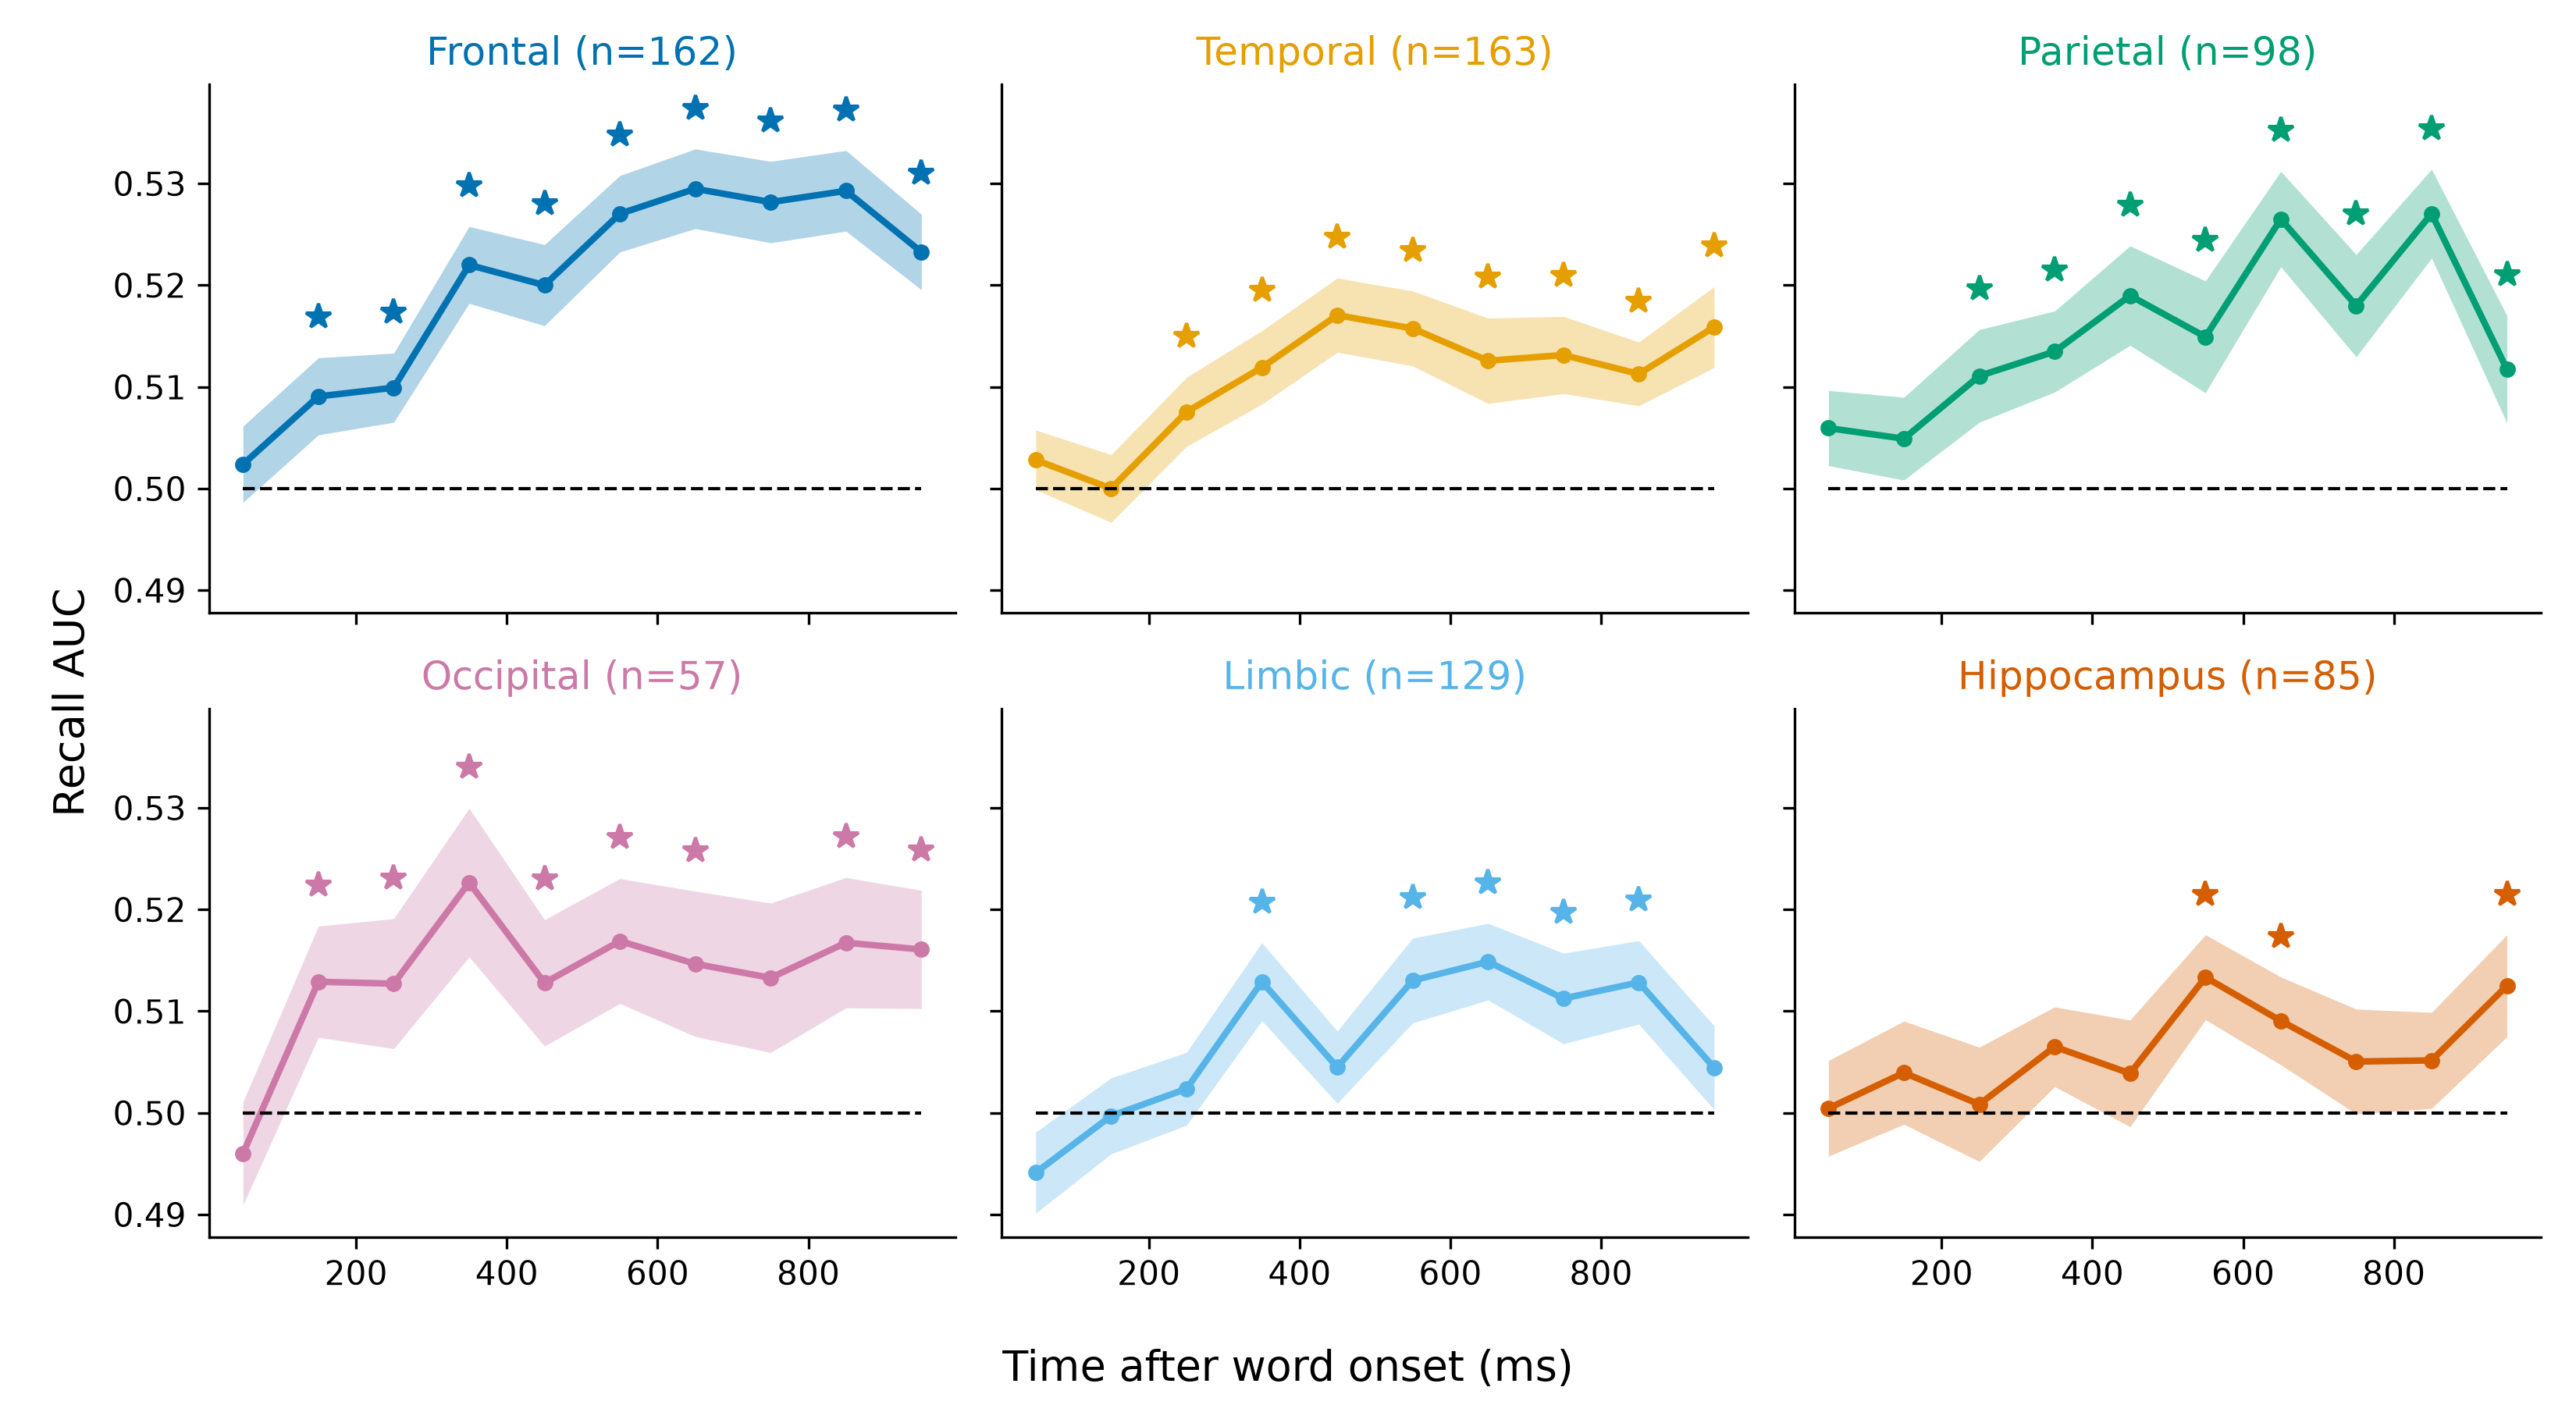
\includegraphics[width=1\linewidth]{img/fig7_recall_time.png}
\caption{Recall prediction from the high-gamma response (encoding contrast: recalled vs.\ not recalled). AUC per lobe and 100 ms window, mean $\pm$ SEM across subjects; dashed line: chance (0.5); stars: AUC above chance, BH-FDR over lobe $\times$ window.}
\label{fig:recall}
\end{figure*}

Frontal regions predict recall in every window from 100 to 1000 ms (Figure~\ref{fig:recall}; peak AUC 0.529 at 600--700 ms) and occipital regions in all but one (100--700 and 800--1000 ms; peak 0.523 at 300--400 ms). Parietal regions predict recall from 200 ms (peak 0.527 at 800--900 ms), temporal regions from 200 ms (peak 0.517 at 400--500 ms), limbic regions at 300--400 and 500--900 ms (peak 0.515 at 600--700 ms), and hippocampus at 500--700 and 900--1000 ms (peak 0.513 at 500--600 ms). No lobe predicts recall at 0--100 ms, before the high-gamma response begins (${\sim}$120 ms). AUCs were low ($\leq$ 0.53) because each classifier used one lobe's high gamma in one 100 ms window, and every electrode in the lobe was one feature. This early-posterior, late-frontal order matches the subsequent memory effect in high-frequency activity \citep{Burke_2014a}.

\subsection*{6. Reliability across
sessions}\label{reliability-across-sessions}

\begin{figure*}[!tp]
\centering
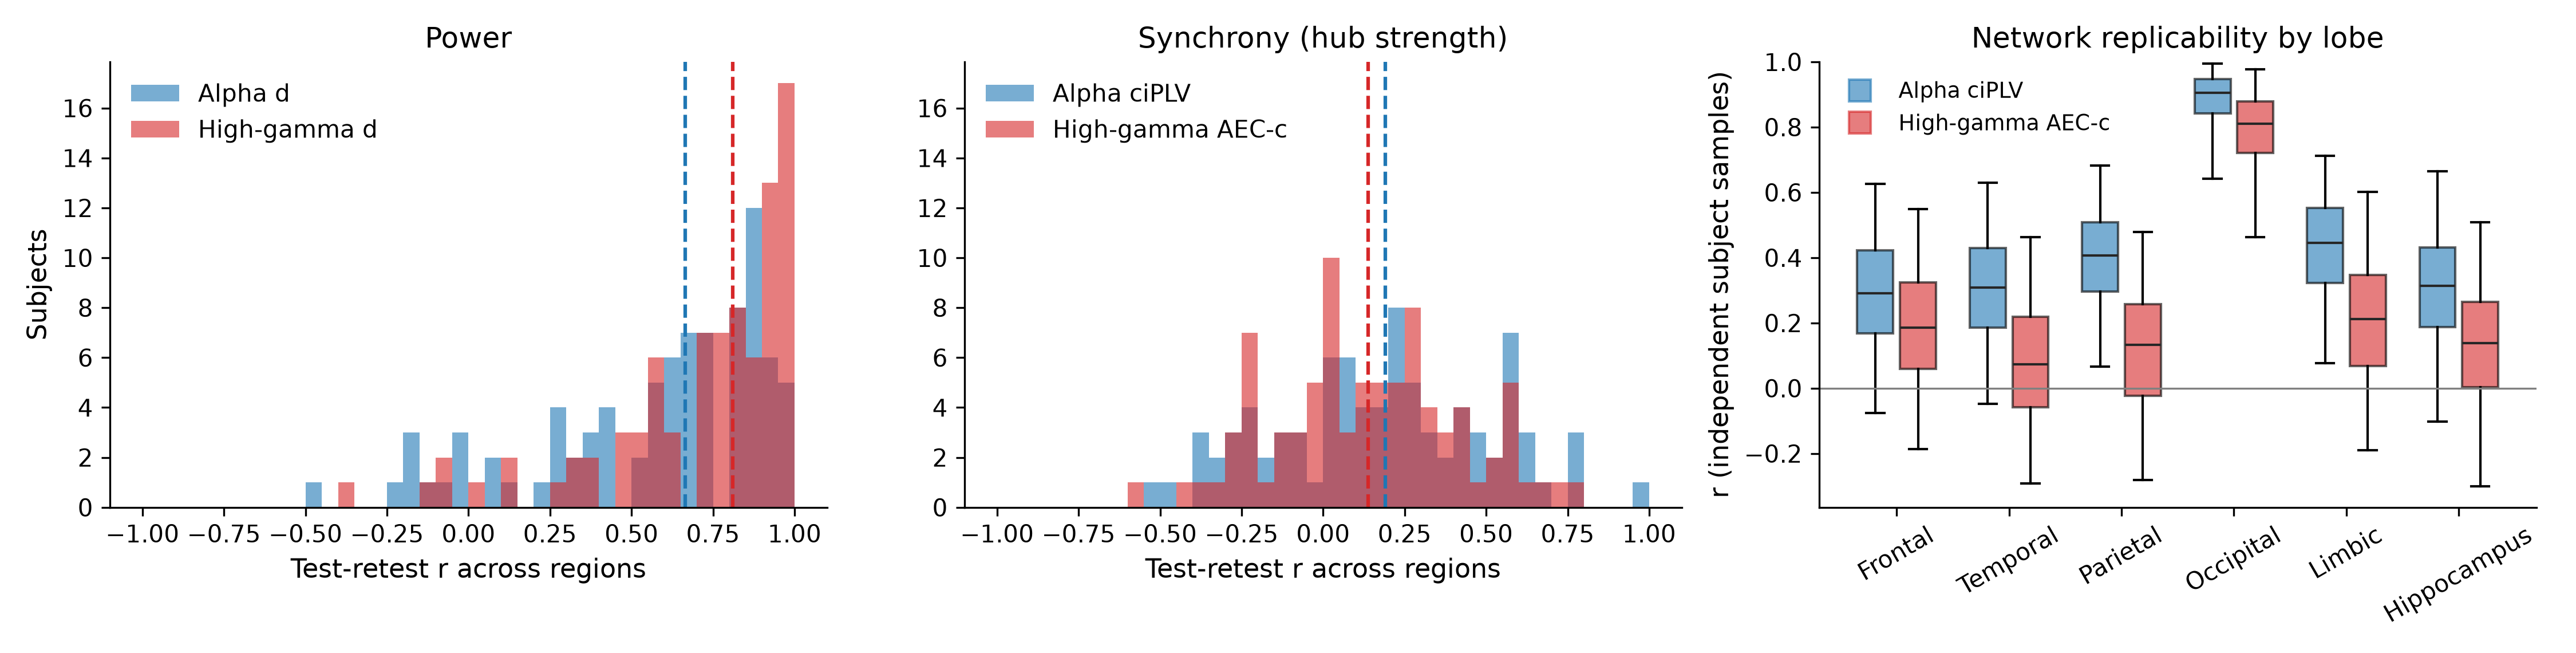
\includegraphics[width=1\linewidth]{img/fig8_reliability.png}
\caption{Session-to-session reliability (left) per subject, Pearson r across regions between two random halves of the subject's sessions, for power (Cohen's $d$) and connectivity hub strength; box plots across subjects (whiskers: central 95\%). (Right) Replicability across subjects of each lobe's connectivity profile: its change on each connection $\times$ window, hemispheres pooled, correlated between two disjoint halves of the subjects (127 each); box plots over 1000 splits (whiskers: central 95\%).}
\label{fig:reliability}
\end{figure*}

Power is reliable across sessions (Figure~\ref{fig:reliability}, left; 91 subjects with at least two sessions per half): median $r$ = 0.67 [IQR 0.38, 0.85] for alpha and 0.81 [0.58, 0.93] for high gamma. Synchrony was much less reliable, with a quarter of subjects below zero (median $r$ = 0.19 [$-0.05$, 0.43] for alpha ciPLV, 0.14 [$-0.04$, 0.32] for high-gamma AEC-c).

Across subjects (right; 127 subjects per half), occipital cortex's connectivity profile replicates well (median $r$ = 0.90 [central 95\% of splits 0.81, 0.95] for alpha, 0.81 [0.64, 0.90] for high gamma), while every other lobe replicated weakly (alpha $\approx$0.3--0.4, intervals excluding 0 only in parietal and limbic cortex; high gamma $\approx$0.1--0.2, all intervals including 0). Occipital replicability stayed at 0.89 after removing each window's mean, so it reflects the pattern over connections, not only a shared time course. In the other lobes, replicability came largely from their connection with occipital cortex. Without it, alpha $r$ fell from 0.43 to 0.17 in limbic cortex and from 0.32 to 0.03 in hippocampus, and remained weak in frontal (0.28), parietal (0.35) and temporal cortex (0.22).

\section*{Discussion}\label{discussion}

The occipital alpha decrease and HG increase match the activation response first described in sensorimotor cortex \citep{Crone_1998a,Crone_1998b} and in visual cortex \citep{Lachaux_2005}, including for pseudowords and consonant strings, where the electrodes selective in each band overlapped little \citep{Vidal_2010}. The same low-frequency decrease and HFA increase marks successful encoding \citep{Sederberg_2003,Long_2014}, and this broadband tilt also appears outside memory, during arithmetic \citep{Randazzo_2019}, where it predicts response speed, mainly in frontal regions \citep{DeHaan_2025}. The frontal low-frequency increase and beta decrease, without a frontal HG increase, fit active suppression of cortex not needed for the task \citep{Jensen_2010}; HG similarly decreases during tasks in default-mode regions \citep{Ossand_n_2011}.

Our latencies agree with smaller iEEG studies. Gamma activity begins at about 150 ms in basal temporal cortex, reaches the VWFA at about 200 ms, and reaches superior temporal and Broca's areas after 400 ms \citep{Mainy_2007}; word-selective ventral temporal electrodes respond at about 150 ms \citep{Kadipasaoglu_2016}; and the effects of word properties move anteriorly along the ventral stream, with feedback to posterior regions at 250--500 ms \citep{Woolnough_2020}. Beyond the ventral stream, MEG shows responses proceeding from temporal cortex to Broca's area and finally to orbitofrontal cortex at about 370 ms \citep{Halgren_2002}, the same order we find. The sharp early and broad late responses we observe are consistent with feedforward input followed by feedback \citep{Halgren_2006,Ghuman_2014}.

While we observe a substantial decrease in alpha power in the occipital cortex, its alpha synchrony with other regions rises, consistent with \citep{Hanslmayr_2016}. Synchrony measured at stimulus onset is, however, harder to interpret than power: an evoked response shared across regions can raise phase and envelope coupling without any interaction between them, and cannot be cleanly separated from cognitive effects \citealp{David_2006,Shah_2004}. Subtracting the average evoked response does not fully remove it, because its amplitude and latency vary across word presentations \citep{Truccolo_2002,David_2006}. The absence of HG envelope coupling is consistent with HFA being local and asynchronous; studies of memory show that regions with gamma increases during successful encoding lose global synchrony \citep{Burke_2013}. 
  %Alternatives to subtraction:
  %Matched condition contrast with a label-shuffle null: \citealp{Solomon_2017,Maris_2007a}.
  %Trial-shuffled (shift-predictor) surrogates: ��Perkel_1967,Aertsen_1989,Brody_1999b.
  %Connectivity aligned to internal HFA peaks: ��Dede_2025.
  % Phase consistency on the same data: ��Colyer_2025.

\subsection*{Expectation}\label{disc-expectation}

Temporally expected events evoke larger visual responses: in monkey V1, gamma increases and alpha decreases when a stimulus is expected \citep{Lima_2011}, and expectation speeds and enhances visual processing in humans \citep{Doherty_2005}. The larger occipital response after longer ISIs fits this account. Because long- and short-ISI events were measured against the same baseline, averaged over all events, the effect cannot come from a raised baseline after short ISIs; an alternative is that the visual response recovers less from the previous word when the interval is short.

\subsection*{Recall prediction}\label{disc-recall}

Recall prediction appeared only after the early visual response, briefly in occipital cortex and persistently in frontal cortex, in the same direction as the early posterior and late frontal HFA effects found by comparing recalled with forgotten words \citep{Burke_2014a}. These classifiers may partly track general fluctuations in brain state rather than encoding of the item \citep{Weidemann_2021}.

\subsection*{Limitations}\label{limitations-discussion}

\begin{itemize}
\tightlist
\item
  Word-off baseline starts \textasciitilde80-410 ms after the previous
  word's offset: possible offset response / anticipation in the
  baseline; the ISI analysis (Results 4) uses one
  baseline averaged over all events and is not affected by it.
\item
  Evoked and induced activity 
\item
  Neighbour-transferred labels (\textasciitilde11\% / 21\% disagreement
  in LOSO) only for the 13\% of unlabelled depth pairs the imaging-pipeline label files
  lack.
\item
  High-gamma phase metrics avoided (broadband HFA has no meaningful
  phase); AEC-c null is consistent with high gamma being local and
  asynchronous \citep{Solomon_2017,Solomon_2019a}.
  \item 
\item
  Multiple comparisons corrected within figures, not across.
\end{itemize}


\onecolumn  % new page, all pending figures printed first
\makeatletter  % LaTeX keeps the last figure page's reduced column height; reset it
\global\@colht\textheight \global\@colroom\textheight \global\vsize\textheight
\makeatother
\renewcommand{\bibsection}{}
\begin{multicols}{2}[\section*{References}]  % references in their own two-column block
\bibliography{refs}
\end{multicols}

\onecolumn  % supplementary in one column so the heading stays with its figures
\section*{Supplementary}\label{supplementary}

\begin{figure}[H]
\centering
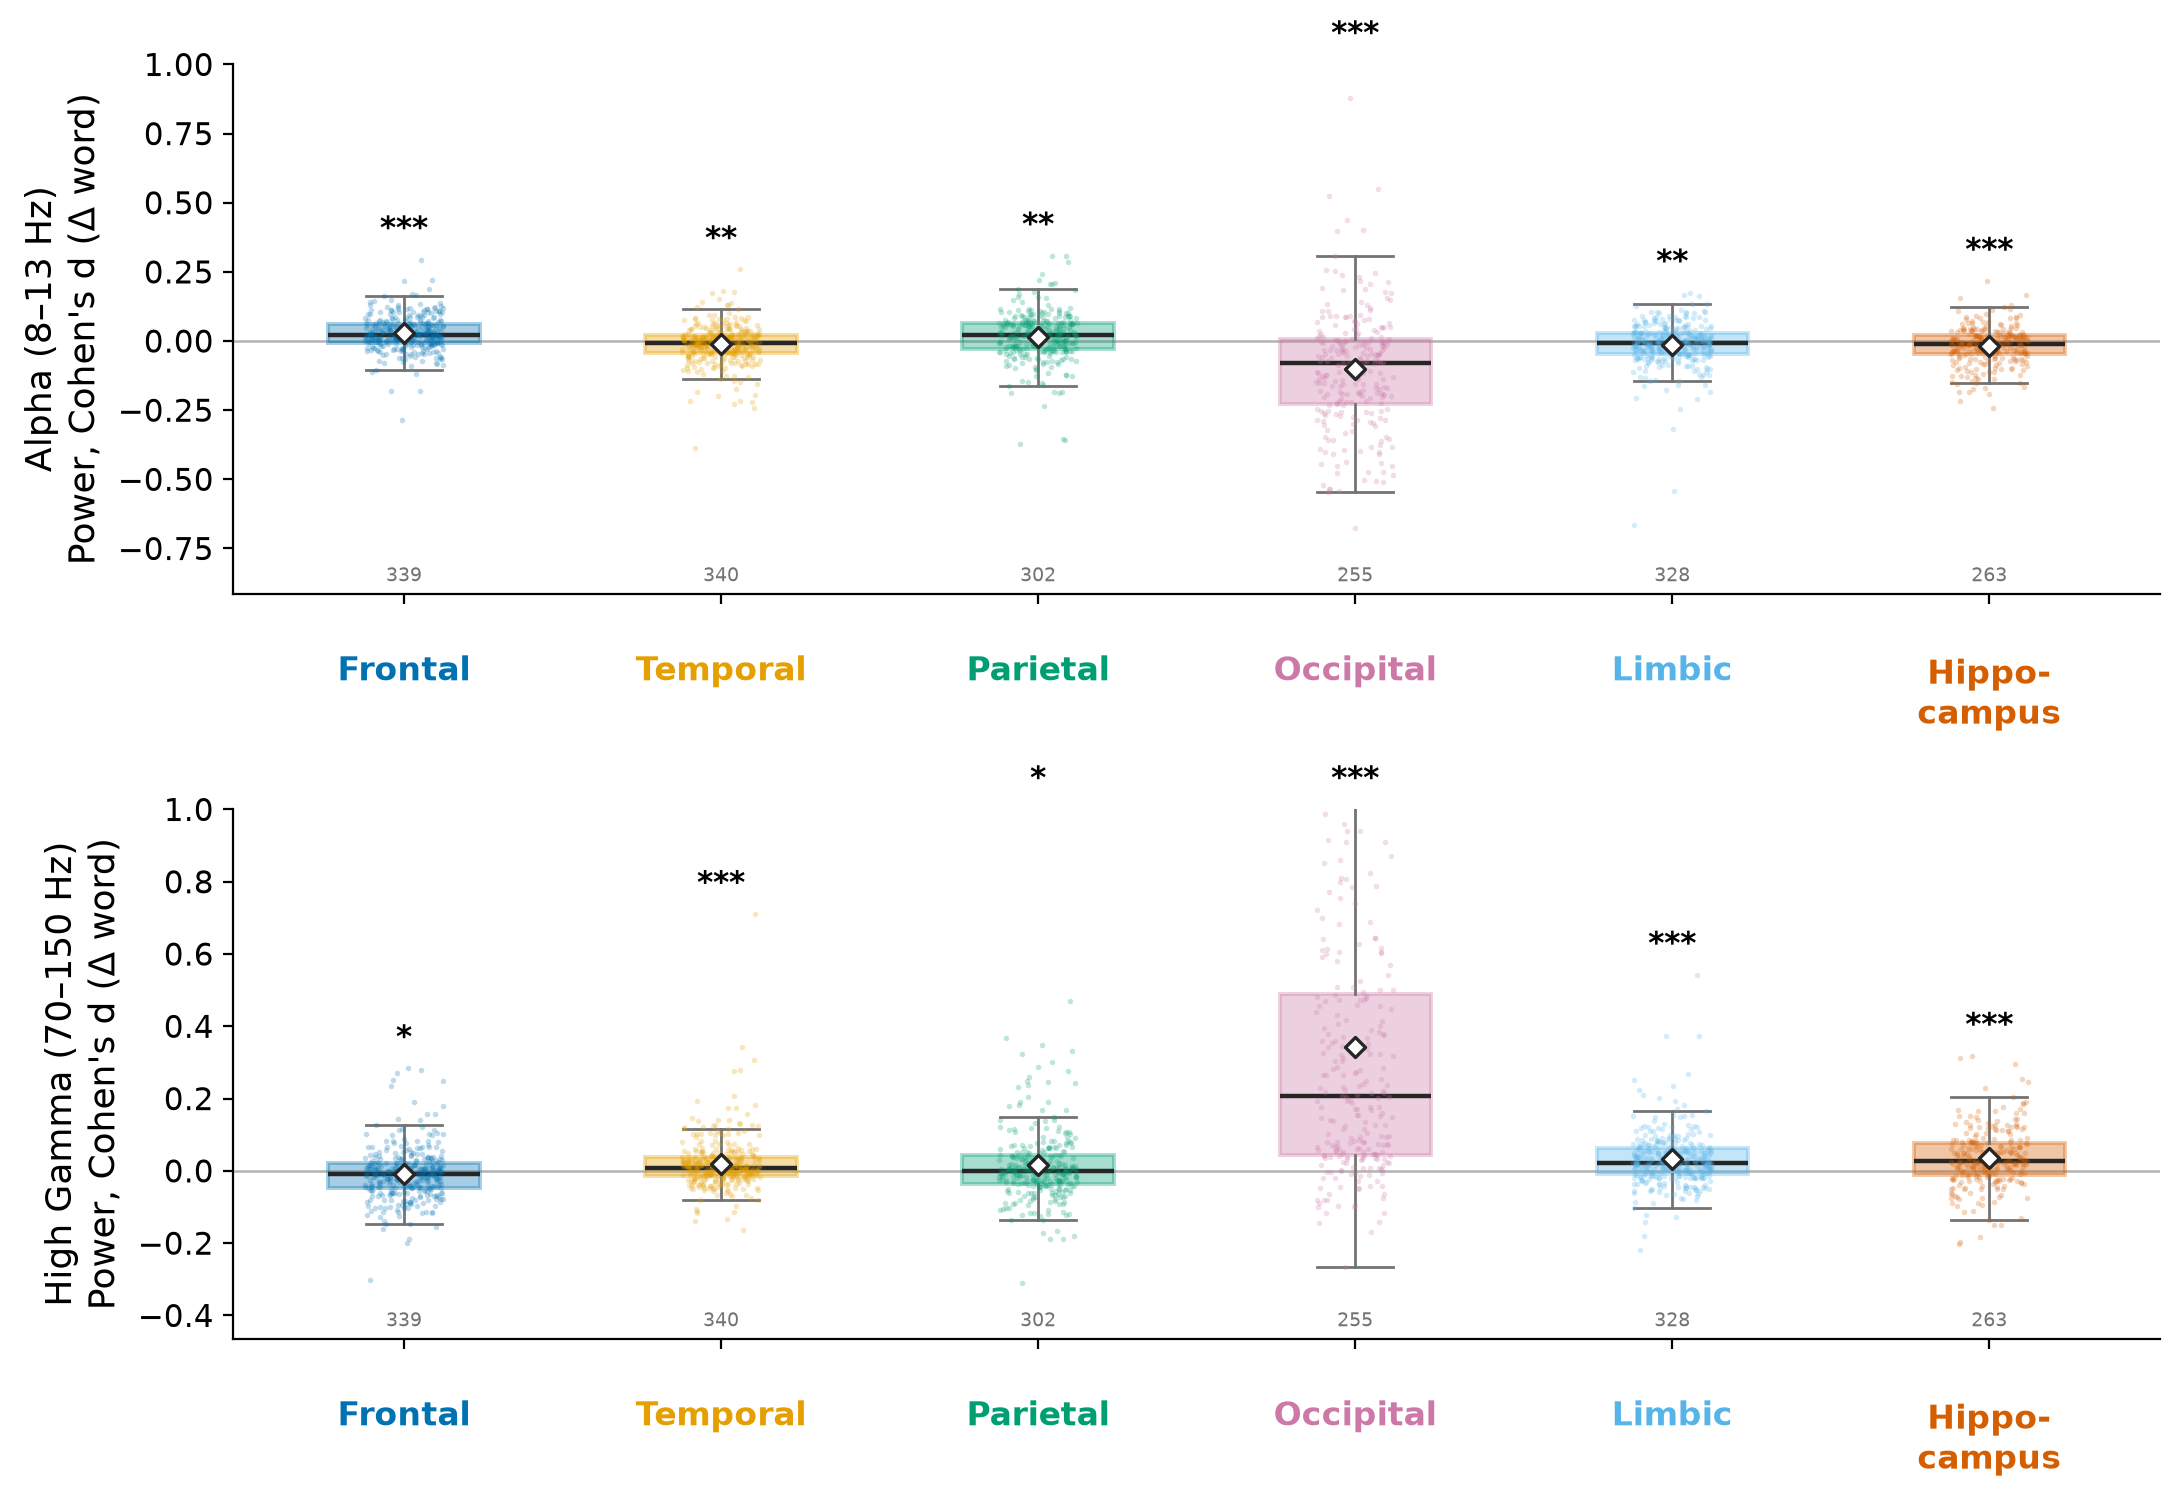
\includegraphics[width=0.8\linewidth]{img/figS1_power_subjects.png}
\caption{Power change per region, subject distributions.}
\end{figure}

\begin{figure}[H]
\centering
\includegraphics[width=0.8\linewidth]{img/figS2_synchrony_subjects.png}
\caption{Synchrony change per region, subject distributions.}
\end{figure}

\begin{figure}[H]
\centering
\includegraphics[width=0.75\linewidth]{img/figS3_spectrum_fine.png}
\caption{Spectral profile per anatomical subregion: t across subjects per subregion and frequency, as in Figure~\ref{fig:power}B, for the 31 subregions recorded in at least 30 subjects (hemispheres pooled; n: subjects), grouped and coloured by region; outlines enclose significant cells (BH-FDR $q<.05$ over all subregions and frequencies).}
\label{fig:spectrum-fine}
\end{figure}

\begin{figure}[H]
\centering
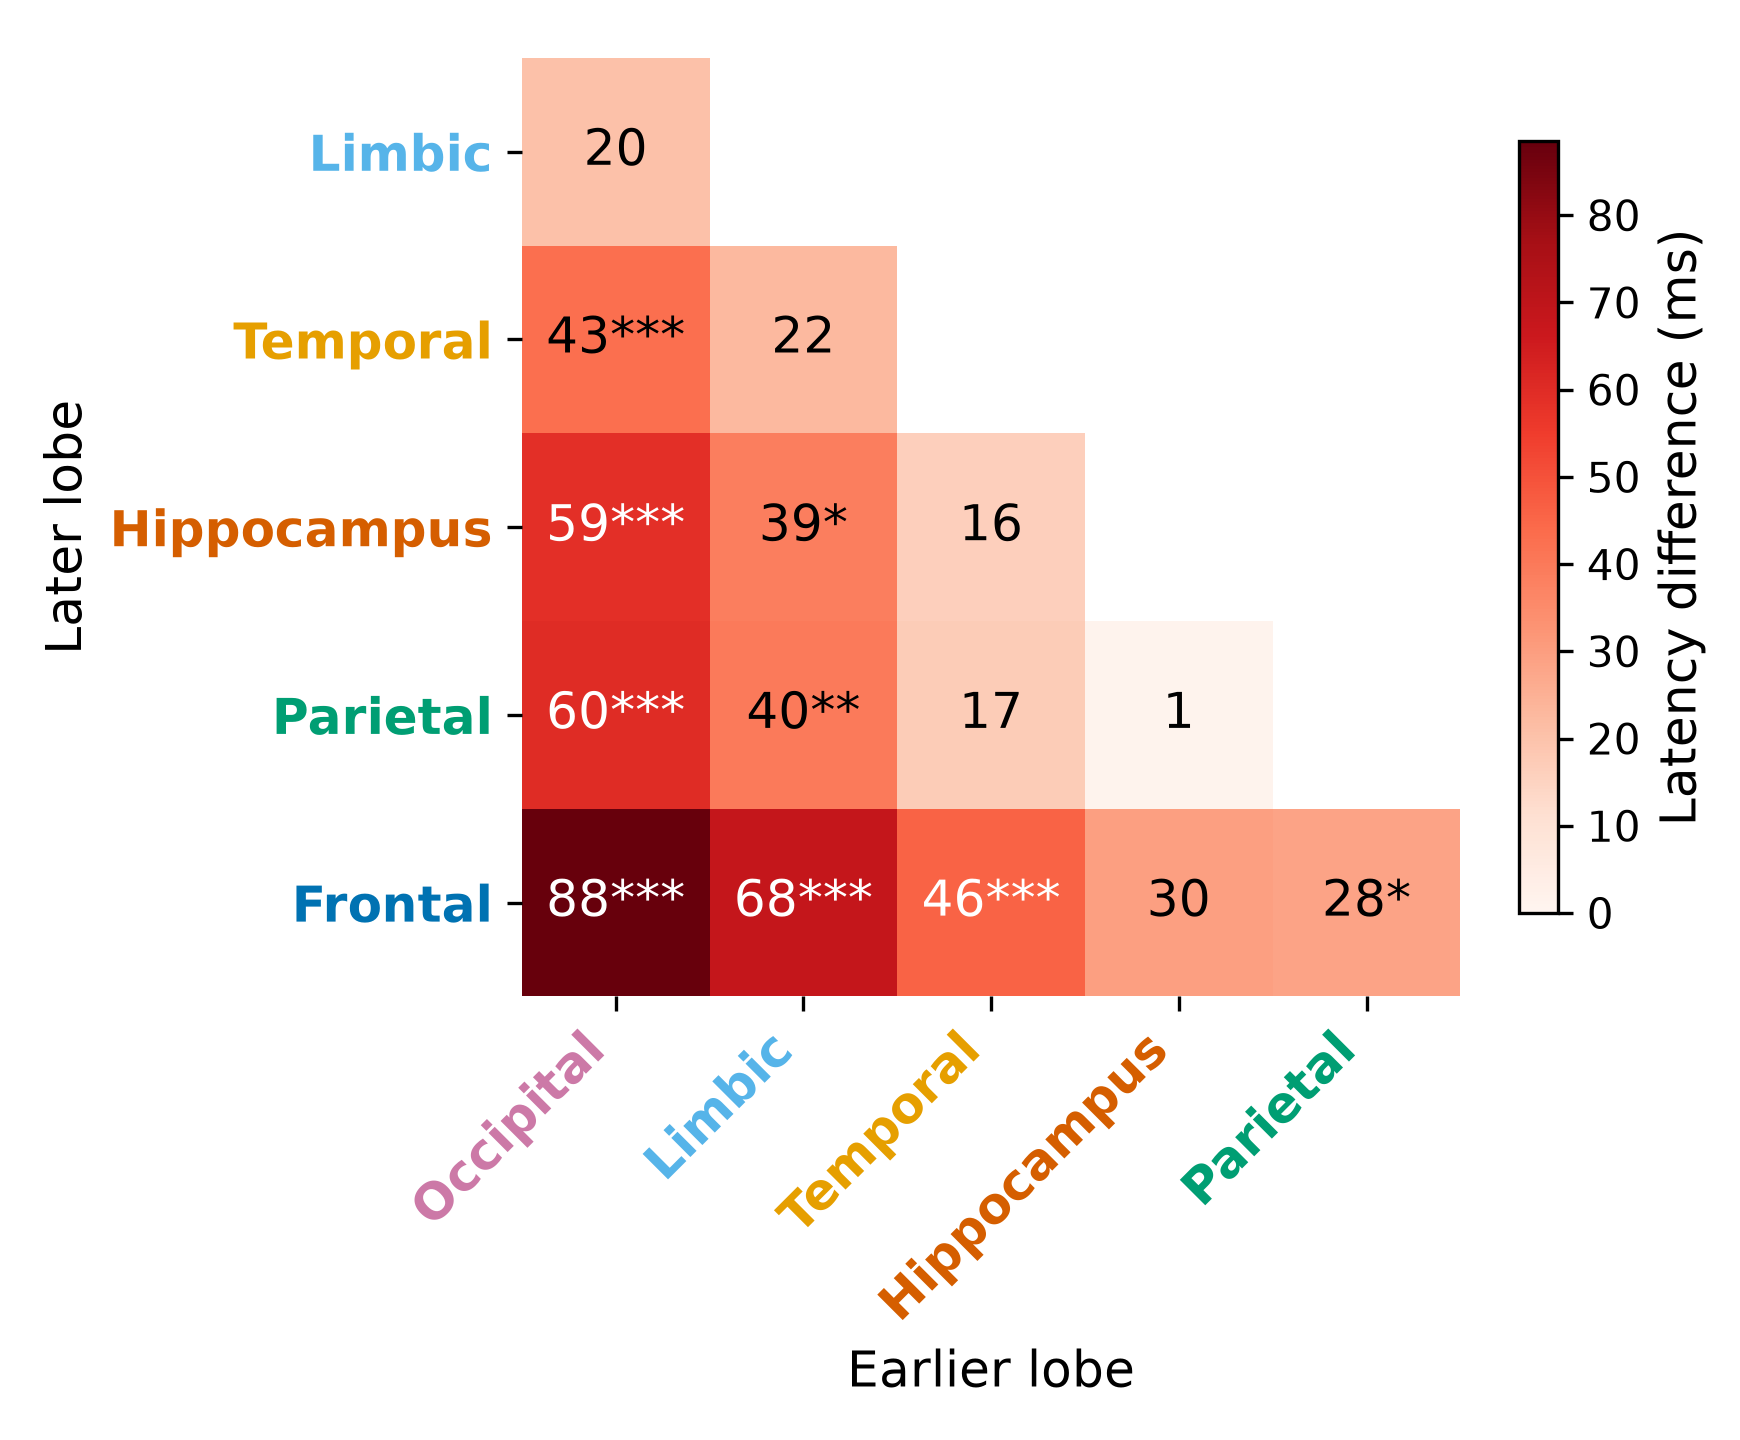
\includegraphics[width=0.6\linewidth]{img/figS5_latency_mixed.png}
\caption{High-gamma latency differences between lobes from the mixed-effects model. Lobes are in latency order (estimated latencies: occipital 150 ms, limbic 170, temporal 193, hippocampus 209, parietal 210, frontal 238 ms); each cell is the row lobe's latency minus the earlier column lobe's (ms); stars: z tests, Holm-corrected over the 15 pairs.}
\label{fig:latency-mixed}
\end{figure}

\begin{figure}[H]
\centering
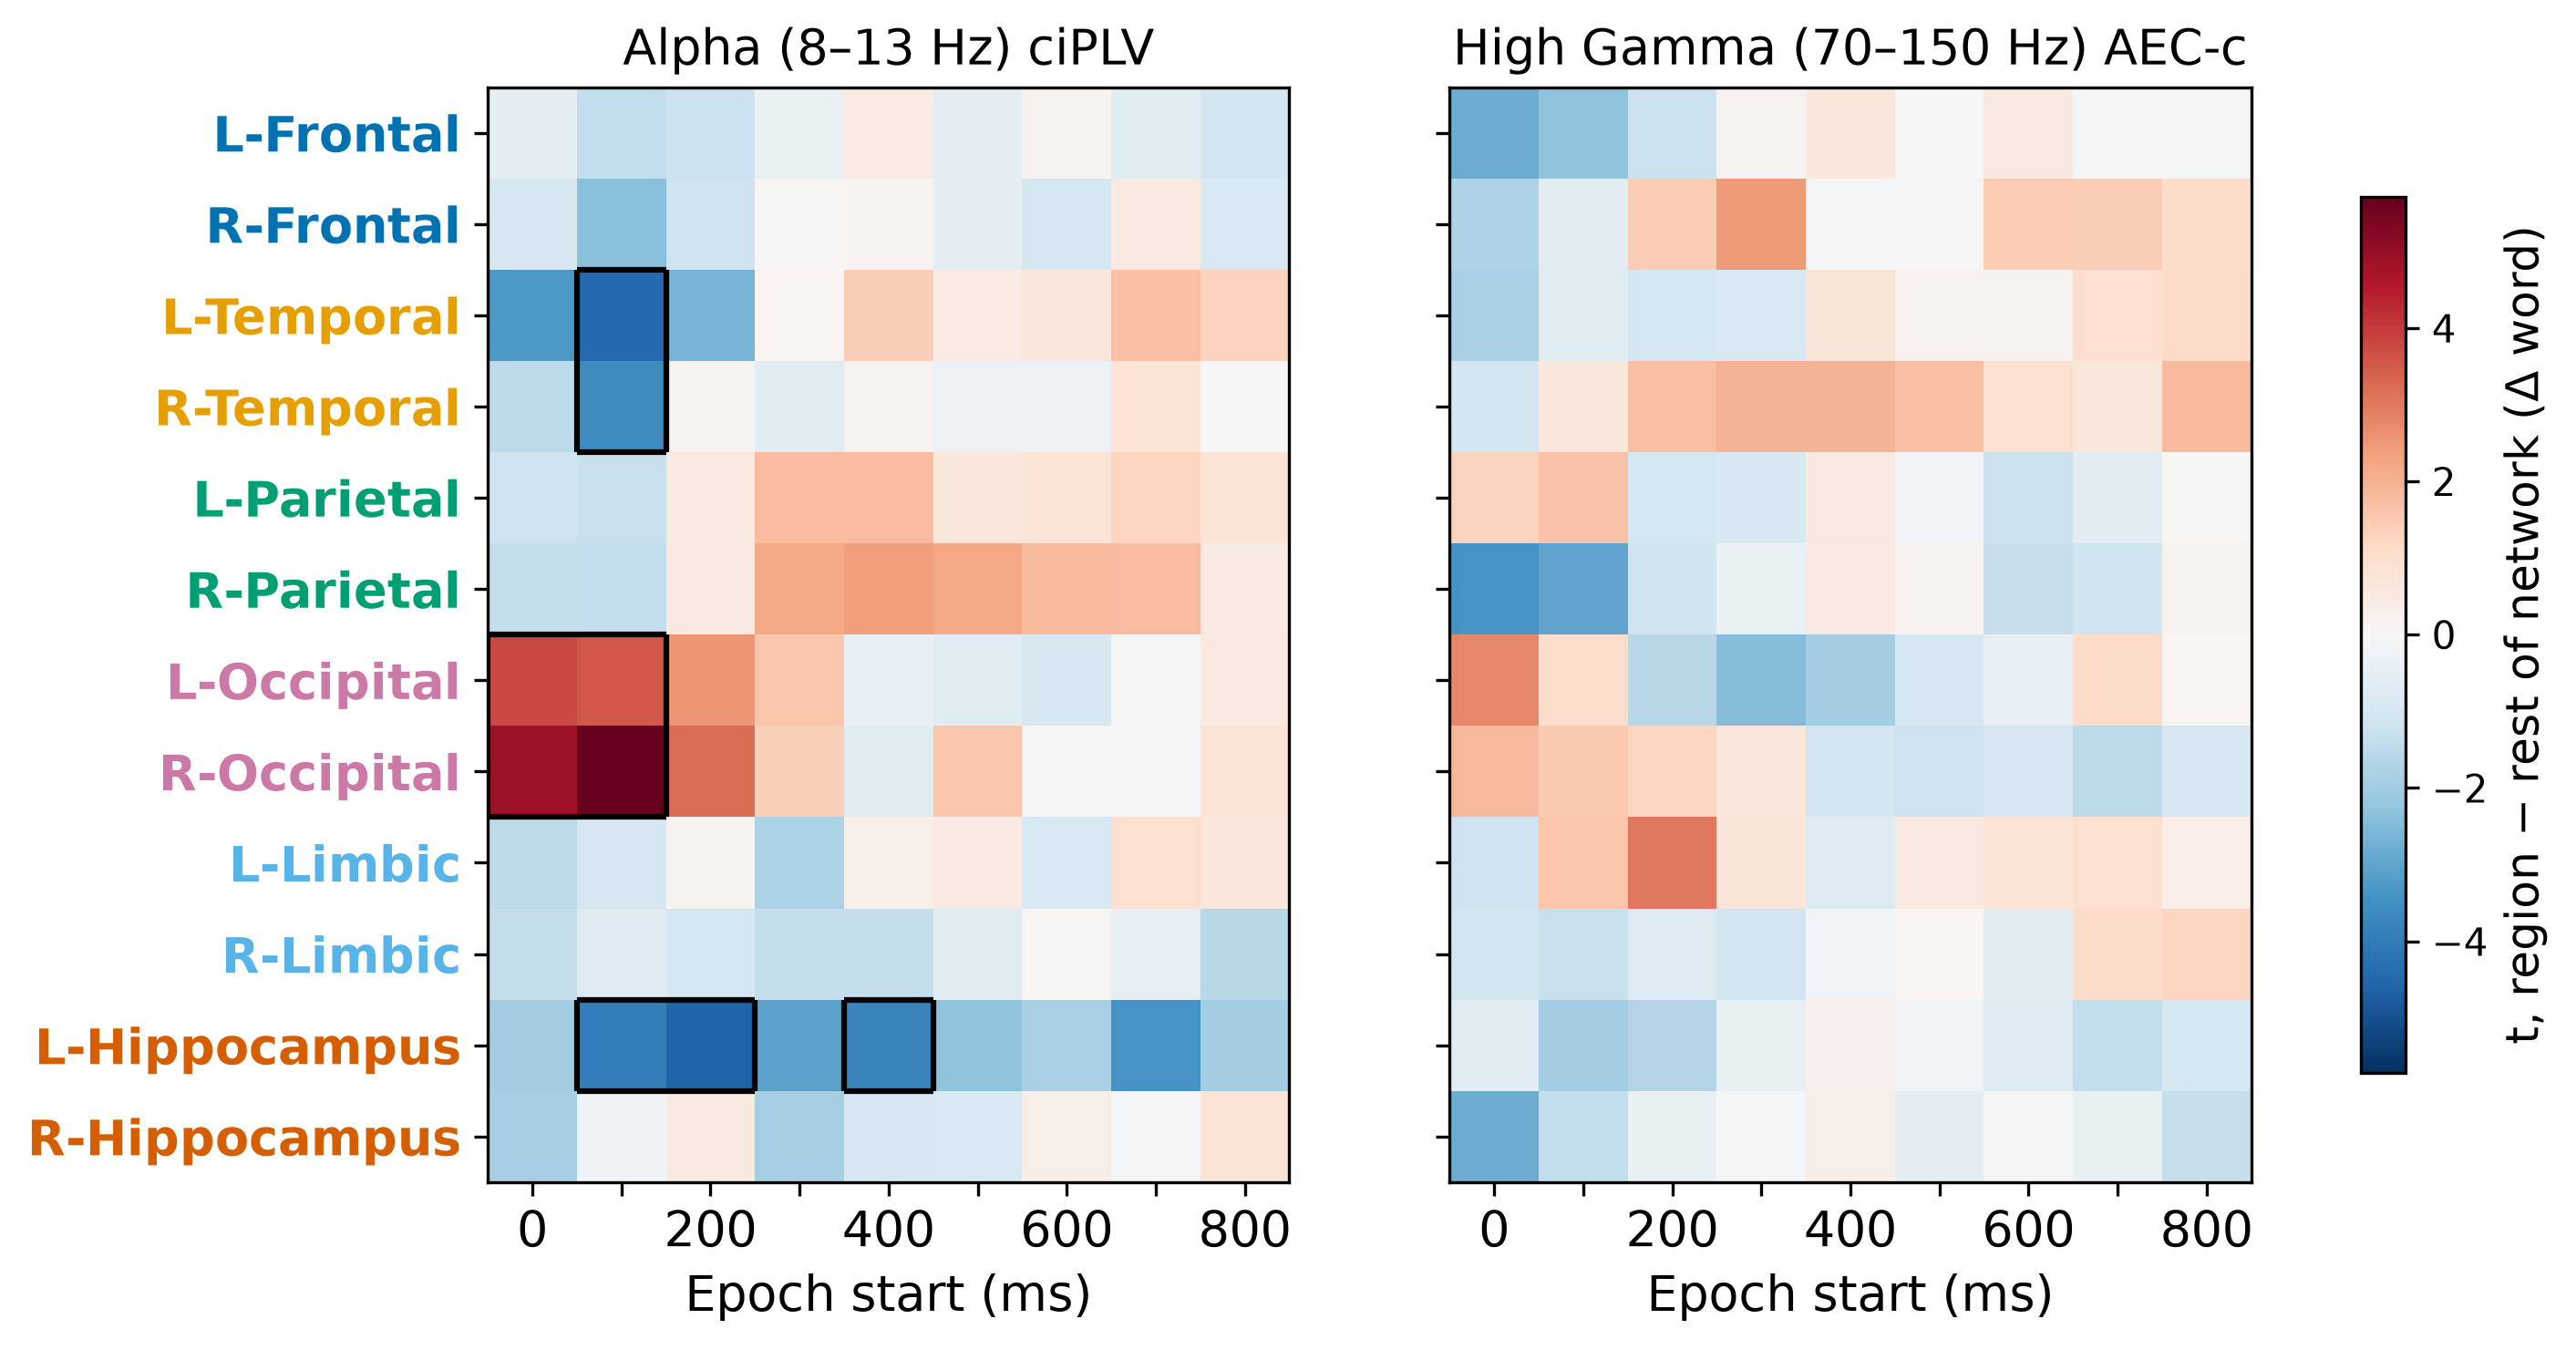
\includegraphics[width=0.8\linewidth]{img/figS6_hubs_relative.png}
\caption{Regions that stand out from the network-wide change in synchrony. Per region and 200 ms window (start shown): $t$ across subjects of the region's mean change over its connections minus the mean change over all connections not involving it, for alpha ciPLV (left) and high-gamma AEC-c (right). Outlines: Holm $p<.05$ over regions $\times$ windows.}
\label{fig:hubs-relative}
\end{figure}






\end{document}
